\documentclass[10pt,a4paper]{article}
\usepackage[margin=2.0cm]{geometry}
\usepackage{graphicx}
\usepackage{amsmath,amssymb}
\usepackage{booktabs}
\usepackage{array}
\usepackage{caption}
\usepackage{microtype}
\usepackage{xcolor}
\usepackage{listings}
\usepackage[colorlinks=true,linkcolor=blue,urlcolor=blue]{hyperref}
% XeLaTeX only (the author line has Chinese characters): fontspec + an installed CJK font, no ctex package needed
\usepackage{fontspec}
\newfontfamily\cjkfont{Noto Serif CJK TC}

% code style: commands to run are shaded boxes with a blue bar; file names and code are teal monospace
\definecolor{codebg}{RGB}{243,245,248}
\definecolor{codebar}{RGB}{60,110,180}
\definecolor{codecomment}{RGB}{120,120,120}
\definecolor{codename}{RGB}{0,110,110}
\lstdefinestyle{cmd}{basicstyle=\ttfamily\footnotesize, backgroundcolor=\color{codebg}, frame=leftline,
  framerule=2.5pt, rulecolor=\color{codebar}, framesep=6pt, xleftmargin=10pt, aboveskip=4pt, belowskip=4pt,
  columns=fullflexible, keepspaces=true, showstringspaces=false, upquote=true,
  morecomment=[l]{\#}, commentstyle=\color{codecomment}\itshape}
\lstnewenvironment{cmd}{\lstset{style=cmd}}{}
\lstnewenvironment{tree}{\lstset{style=cmd, rulecolor=\color{codecomment}}}{}
\AtBeginDocument{\DeclareUrlCommand\path{\def\UrlFont{\color{codename}\ttfamily}}}
\newcommand{\code}[1]{\leavevmode{\color{codename}\ttfamily #1}}
\newcolumntype{L}[1]{>{\raggedright\arraybackslash}p{#1}}

% diagrams: hand-drawn look (slightly wobbly borders, pastel fills)
\usepackage{tikz}
\usetikzlibrary{positioning,arrows.meta,decorations.pathmorphing,calc,fit,backgrounds}
\definecolor{cSyn}{RGB}{70,120,200}
\definecolor{cReal}{RGB}{225,130,40}
\definecolor{cShared}{RGB}{60,150,90}
\definecolor{cOut}{RGB}{140,90,170}
\definecolor{cHold}{RGB}{235,90,80}
\tikzset{
  sketch/.style={decorate, decoration={random steps, segment length=6pt, amplitude=.4pt}},
  box/.style={draw=#1!75!black, fill=#1!13, line width=.7pt, sketch, align=center,
    font=\sffamily\scriptsize, inner sep=3pt, minimum height=9mm, execute at begin node=\hyphenpenalty10000\relax},
  arr/.style={-{Stealth[length=2.2mm]}, line width=.8pt, draw=black!65},
  note/.style={font=\sffamily\scriptsize, align=center, text=black!75},
  holdshape/.pic={\path[pic actions] (-0.34,-0.18) -- (0.34,-0.18) -- (0.25,0.1)
    .. controls (0.2,0.32) and (-0.2,0.32) .. (-0.25,0.1) -- cycle;},
}

\graphicspath{{figures/}}
\captionsetup{font=footnotesize,skip=3pt}
\setlength{\parindent}{0pt}
\setlength{\parskip}{3pt}
\setlength{\emergencystretch}{3em}
\setlength{\textfloatsep}{8pt}

\title{\vspace{-1.8em}Climbing-Hold Detection with Superpixels\\\large Code and workflow documentation\vspace{-0.6em}}
\author{[{\cjkfont 常凱文} 61575082H] \\ \small Computer Vision --- Midterm, National Taiwan Normal University}
\date{\vspace{-0.6em}November 2026}

\begin{document}
\maketitle
\vspace{-2em}

%==========================================================================
\section{About this project}
\label{sec:about}
Given a picture of a climbing wall, the system finds the colored holds and outputs, for each hold, its \emph{type},
its \emph{position} $(x,y,z)$ in meters and its \emph{orientation} (roll, pitch, yaw). It uses the three OpenCV
superpixel algorithms SLIC, LSC and SEEDS and compares them. There are two kinds of input; each has its own code
folder, data and tuned values (the \emph{baseline}).

\begin{center}\small
\begin{tabular}{L{2.6cm}L{6.5cm}L{6.5cm}}
\toprule
 & \textbf{Synthetic walls} & \textbf{Real walls}\\
\midrule
Names & \path{synthetic_wall1} \ldots \path{synthetic_wall4} & \path{real_wall1}, \path{real_wall2}\\
Scale and origin & red square (1~m, 0.1~m on narrow walls) & 20~cm grid of bolt holes\\
Ground truth & \path{scene.json} from the simulator & hand labels (\path{labels.json}, \path{real_wall2})\\
Type / depth $z$ & hold color / stereo pair & nearest labelled color / none ($z=0$)\\
Baseline files & \path{baseline/synthetic_wall_*.json} & \path{baseline/real_wall_*.json}\\
\bottomrule
\end{tabular}
\end{center}
\textbf{How to read this document.} Commands to type in a terminal are in shaded boxes; file names, folder names and
code are in \code{teal monospace}. All commands are run from the project root.

\textbf{Two ways to run every script.} (1) From a terminal, with options (\code{-h} lists them). (2) With the
editor's Run button: every script that takes parameters has a block \code{Run-button settings} (at the top of a wall's
\code{run.py}, at the bottom of the others) with the same options as plain variables, for example
\code{MARKER = 0.1}. The button uses these values; an option typed in a terminal overrides them.

%==========================================================================
\section{Quick start}
\label{sec:quick}
Requirements: Python~3 with the \emph{contrib} build of OpenCV (the superpixels are in \code{cv2.ximgproc}, which
plain \code{opencv-python} lacks); \code{xelatex} only to build this document.
\begin{cmd}
pip install opencv-contrib-python numpy matplotlib
\end{cmd}

\subsection{Add a new synthetic wall}
\label{sec:newsyn}
There are two ways to use a new wall. \textbf{Path A} only \emph{tests} the existing baselines on it.
\textbf{Path B} lets the wall take part in choosing the baselines. Do Path~A first: once the wall is part of the
choice, its score is no longer a fair test.

\textbf{Step 0: add the files.} Create \path{dataset/synthetic_wall4/} with:

\begin{center}\small
\begin{tabular}{L{3.8cm}L{1.6cm}L{10.2cm}}
\toprule
File & Required & Notes\\
\midrule
\path{wall.png} or \path{image.png} & yes & main camera view; the \emph{whole} red square must be visible\\
\path{scene.json} & yes & ground truth; also gives the marker size (\code{scene.wall.originMarker.width})\\
\path{stereo.png} & no & left eye $|$ right eye side by side; without it $z=0$\\
\path{camera.json} & no & stereo camera height and distance, read from the simulator page:
 \code{\{"stereo": \{"height\_m": 0.7, "distance\_m": 1.0\}\}}\\
\bottomrule
\end{tabular}
\end{center}

\textbf{Path A: held-out test} (``how good are the frozen baselines on a wall they never saw?'')
\begin{cmd}
python3 src/pipelines/synthetic_wall/new_wall.py synthetic_wall4   # 1. create the wall's run script
python3 outputs/synthetic_wall4/scripts/run.py                     # 2. run SLIC, LSC and SEEDS on it
\end{cmd}
Step 1 checks the dataset folder and writes \path{outputs/synthetic_wall4/scripts/run.py}, a small wrapper you do not
edit. Step 2 reads the baselines from \path{baseline/synthetic_wall_algorithm.json} \emph{without changing them} and
writes \path{outputs/synthetic_wall4/<algo>/}. Open \code{detections.png} there (green = true hold found, red = false
positive). The printed output has three parts: the new wall alone; a table of \emph{every} wall (old walls are read
from their saved \code{score.json}; read the \code{synthetic\_wall4} rows, not the \code{all} rows); and the refreshed
sweep summary, where only the new wall is computed (about 1~s) and the baseline is untouched.
Options (terminal) or variables at the top of \code{run.py} (Run button): \code{--algo} / \code{ALGO = "slic"},
\code{--thresh}, \code{--min-sat} (override the baseline for this run), \code{--stereo-height},
\code{--stereo-distance} (no \code{camera.json}), \code{--marker} / \code{MARKER = 0.1} (only if \code{scene.json}
lacks the marker size), \code{--no-pooled}, \code{--force}.

\textbf{Path B: let the wall join the choice.} This overwrites the baseline, so every number in this document can change.
\begin{cmd}
python3 src/pipelines/synthetic_wall/run_all.py                    # sweep, pick, run, compare
python3 src/pipelines/synthetic_wall/run_all.py --keep-baseline    # same, but keep the baseline file
\end{cmd}
It does five steps: (1) \textbf{sweep}: only the new wall is computed, the others are cached, all are joined in
\path{outputs/synthetic_wall_sweep/sweep_all.csv}; (2) \textbf{best}: the best setting per algorithm is chosen again
(Section~\ref{sec:select}) and \path{synthetic_wall_algorithm.json} is overwritten; (3) \textbf{run} every wall with
every algorithm; (4) \textbf{compare}: print the table; (5) \textbf{yaw}: redraw \path{synthetic_wall_yaw_examples.png}.
With \code{--keep-baseline} step 2 is skipped; the summary then says ``the sweep now prefers \ldots'' if a better
setting exists. Afterwards rebuild the figures and this document (the numbers in the text are typed by hand):
\begin{cmd}
python3 src/pipelines/make_report_figures.py
cd report && latexmk -xelatex main.tex
\end{cmd}

\subsection{Add a real wall photo}
\label{sec:newreal}
\begin{cmd}
python3 src/pipelines/real_wall/calibrate_grid.py real_wall3     # photo in dataset/real_wall3/image.png
python3 src/pipelines/real_wall/run_wall.py real_wall3           # all algorithms (or add: lsc)
\end{cmd}
Check \path{outputs/real_wall3/calibration.png}: the magenta grid must lie on the bolt holes and the median residual
should be about 1~px. The detector then runs with the frozen real baseline. Only \path{real_wall2} has labels, so the
score of a new photo means something only if it shows the same wall (labels are carried over by whole grid cells);
otherwise judge \code{detections.png} by eye. To tune on another photo, label it in \path{labels.json}
(\code{\{"holds": [\{"id": "hold\_0", "pixel": [190, 120], "color": "green"\}, ...]\}}), set \code{labels\_wall} and
\code{test\_wall} in \path{real_wall_parameters.json} and run the real sweep with \code{--save-best}.

\subsection{Other tasks}
\begin{cmd}
python3 src/pipelines/run_all.py                           # everything, synthetic then real (about 1 minute)
python3 src/pipelines/synthetic_wall/sweep.py --save-best  # re-tune the synthetic baseline only
python3 src/pipelines/real_wall/sweep.py --save-best       # re-tune the real baseline only
python3 src/pipelines/synthetic_wall/sweep.py --replot     # redraw the plots from the saved csv
\end{cmd}
Fixed values (window, size limits, scale, stereo, yaw, grid) are edited by hand in
\path{baseline/*_parameters.json}; the tuned values (size, $T$, $S$) are never edited by hand, only re-tuned.
The sweep grid is \code{SIZES}, \code{THRESH}, \code{SATS} at the top of each \code{sweep.py}. A new superpixel
algorithm is a new case in \code{segment()} and a name in \code{ALGOS} (\path{src/shared/superpixels.py}); every loop
goes over \code{ALGOS}, so it gets its own baseline and folders.

\subsection{Build this document (note for later)}
The document is compiled with \textbf{XeLaTeX}, because the author line has Chinese characters: XeLaTeX can use any
installed font through \code{fontspec}, here \emph{Noto Serif CJK TC} (\code{\textbackslash newfontfamily\textbackslash
cjkfont} in the preamble). This avoids the \code{ctex} package, which needs the large \code{texlive-lang-chinese};
plain \code{pdflatex} cannot typeset the Chinese characters. On Ubuntu/Debian:
\begin{cmd}
sudo apt install texlive-xetex texlive-latex-recommended latexmk   # LaTeX compiler and the packages used here
sudo apt install fonts-noto-cjk                                    # Chinese/Japanese/Korean fonts
fc-list | grep "Noto Serif CJK TC"                                 # check that the font is found
\end{cmd}
Then compile; \code{latexmk} reruns XeLaTeX until the references are right, \code{-c} removes the helper files:
\begin{cmd}
cd report
latexmk -xelatex main.tex                                  # writes main.pdf
latexmk -xelatex -interaction=nonstopmode main.tex         # same, never stops to ask on an error
latexmk -c                                                 # clean up .aux .log .xdv ...
\end{cmd}
If it stops with \code{File `xxx.sty' not found}, a LaTeX package is missing: type \code{X} and Enter to quit, find
the Debian package with \code{apt-file search xxx.sty} and install it. Errors are explained in \path{report/main.log}.
On Windows or macOS, install TeX Live or MiKTeX (both include XeLaTeX and \code{latexmk}) and any Noto CJK font.

%==========================================================================
\section{Project layout}
\label{sec:layout}
\begin{tree}
baseline/   synthetic_wall_parameters.json  real_wall_parameters.json   # fixed values, by hand
            synthetic_wall_algorithm.json   real_wall_algorithm.json    # tuned values, by the sweep
dataset/    synthetic_wall<N>/  real_wall<N>/                           # input only, never written
outputs/    <wall>/<algo>/  output.json score.json detections.png run.log
            <wall>/sweep.csv  <wall>/scripts/run.py
            synthetic_wall_sweep/  real_wall_sweep/                     # pooled sweep, ROC plots
src/shared/           paths superpixels candidates matching             # used by both kinds of wall
src/synthetic_wall/   baseline calibration evaluate orientation stereo
src/real_wall/        baseline grid_calibration detection
src/pipelines/        run_all make_report_figures                       # the runnable scripts
  synthetic_wall/     run_all sweep run_wall detect stereo_depth final_output new_wall
  real_wall/          run_all calibrate_grid sweep run_wall
\end{tree}
Two rules: the two kinds of wall share \emph{code} (\path{src/shared/}) but no tuned value; \path{dataset/} is only
read, \path{outputs/} only written, and \path{baseline/} changes only when a sweep is run with \code{--save-best}.

%==========================================================================
\section{How the pipeline works}
\label{sec:flow}
Fig.~\ref{fig:pipeline} shows the whole pipeline; blue boxes are synthetic only, orange real only, green shared
(\path{src/shared/}).

\begin{figure}[!htb]
\centering
\resizebox{\linewidth}{!}{%
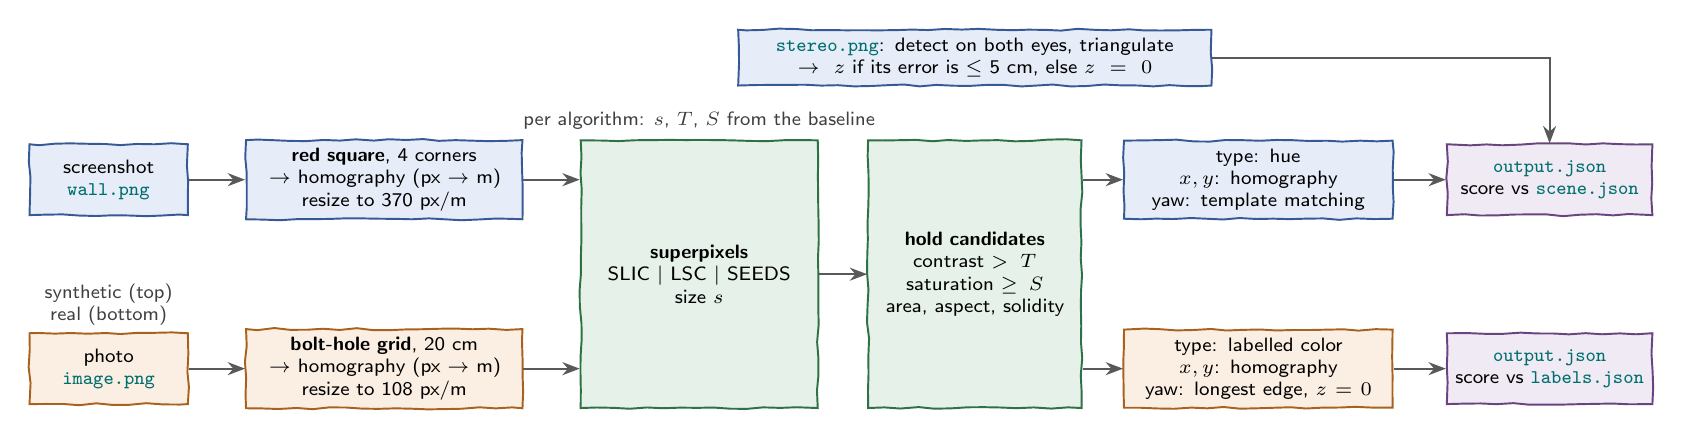
\begin{tikzpicture}
\pgfmathsetseed{3}
\node[box=cSyn, text width=18mm] (inS) at (0,1.2) {screenshot\\\code{wall.png}};
\node[box=cReal, text width=18mm] (inR) at (0,-1.2) {photo\\\code{image.png}};
\node[box=cSyn, text width=33mm] (calS) at (3.5,1.2) {\textbf{red square}, 4 corners\\$\to$ homography (px $\to$ m)\\resize to 370 px/m};
\node[box=cReal, text width=33mm] (calR) at (3.5,-1.2) {\textbf{bolt-hole grid}, 20 cm\\$\to$ homography (px $\to$ m)\\resize to 108 px/m};
\node[box=cShared, text width=28mm, minimum height=34mm] (sp) at (7.5,0) {\textbf{superpixels}\\SLIC $|$ LSC $|$ SEEDS\\size $s$};
\node[box=cShared, text width=25mm, minimum height=34mm] (cand) at (11.0,0) {\textbf{hold candidates}\\contrast $>T$\\saturation $\ge S$\\area, aspect, solidity};
\node[box=cSyn, text width=32mm] (dS) at (14.6,1.2) {type: hue\\$x,y$: homography\\yaw: template matching};
\node[box=cReal, text width=32mm] (dR) at (14.6,-1.2) {type: labelled color\\$x,y$: homography\\yaw: longest edge, $z=0$};
\node[box=cSyn, text width=58mm, minimum height=7mm] (st) at (11.0,2.75) {\code{stereo.png}: detect on both eyes, triangulate\\$\to z$ if its error is $\le$ 5 cm, else $z=0$};
\node[box=cOut, text width=24mm] (oS) at (18.3,1.2) {\code{output.json}\\score vs \code{scene.json}};
\node[box=cOut, text width=24mm] (oR) at (18.3,-1.2) {\code{output.json}\\score vs \code{labels.json}};
\draw[arr] (inS) -- (calS);
\draw[arr] (inR) -- (calR);
\draw[arr] (calS.east) -- (calS.east -| sp.west);
\draw[arr] (calR.east) -- (calR.east -| sp.west);
\draw[arr] (sp) -- (cand);
\draw[arr] (cand.east |- dS.west) -- (dS);
\draw[arr] (cand.east |- dR.west) -- (dR);
\draw[arr] (dS) -- (oS);
\draw[arr] (dR) -- (oR);
\draw[arr] (st.east) -| (oS.north);
\node[note, anchor=south] at (sp.north) {per algorithm: $s$, $T$, $S$ from the baseline};
\node[note, anchor=north] at ($(inS.south)!.5!(inR.north)$) {synthetic (top)\\real (bottom)};
\end{tikzpicture}}
\caption{The pipeline. Each wall is first calibrated to meters and resized to a fixed resolution; the superpixels and
the hold candidates are the same code for both kinds of wall; the description of a hold differs.}
\label{fig:pipeline}
\end{figure}

\begin{figure}[!htb]
\centering
\begin{minipage}[t]{0.32\linewidth}\centering
\resizebox{\linewidth}{!}{%
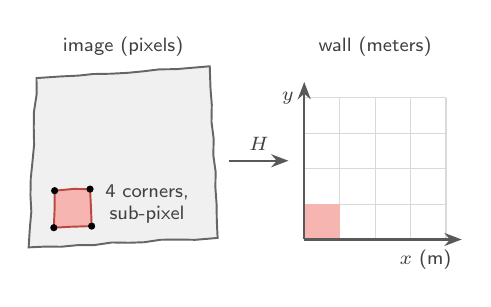
\begin{tikzpicture}
\pgfmathsetseed{5}
\draw[sketch, fill=black!6, draw=black!60, line width=.7pt] (0,0) -- (2.4,0.12) -- (2.3,2.3) -- (0.1,2.15) -- cycle;
\draw[sketch, fill=cHold!45, draw=cHold!80!black, line width=.7pt] (0.32,0.25) -- (0.8,0.27) -- (0.78,0.74) -- (0.33,0.72) -- cycle;
\foreach \p in {(0.32,0.25),(0.8,0.27),(0.78,0.74),(0.33,0.72)} \fill[black] \p circle (1.3pt);
\node[note] at (1.2,2.55) {image (pixels)};
\node[note, anchor=west] at (0.85,0.55) {4 corners,\\sub-pixel};
\draw[arr] (2.55,1.1) -- node[above, note] {$H$} (3.3,1.1);
\begin{scope}[shift={(3.5,0.1)}]
\draw[black!15, step=0.45] (0,0) grid (1.8,1.8);
\fill[cHold!45] (0,0) rectangle (0.45,0.45);
\draw[arr] (0,0) -- (2.0,0) node[below left, note] {$x$ (m)};
\draw[arr] (0,0) -- (0,2.0) node[below left, note] {$y$};
\node[note] at (0.9,2.45) {wall (meters)};
\end{scope}
\end{tikzpicture}}\\[2pt]
{\footnotesize (a) \textbf{Calibration.} The square's corners give a homography; real walls use the 20~cm bolt-hole grid.}
\end{minipage}\hfill
\begin{minipage}[t]{0.32\linewidth}\centering
\resizebox{\linewidth}{!}{%
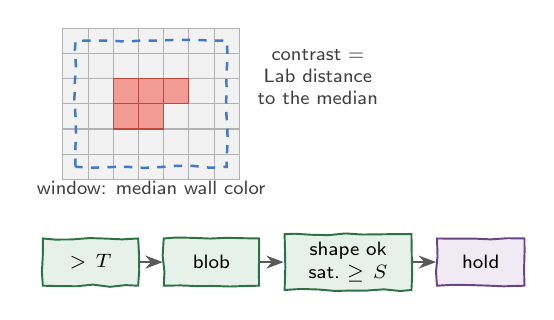
\begin{tikzpicture}
\pgfmathsetseed{7}
\foreach \i in {0,...,6} \foreach \j in {0,...,5}
  \draw[black!30, fill=black!5] (\i*0.32,\j*0.32) rectangle ++(0.32,0.32);
\foreach \i/\j in {2/2,3/2,2/3,3/3,4/3}
  \filldraw[fill=cHold!60, draw=cHold!80!black] (\i*0.32,\j*0.32) rectangle ++(0.32,0.32);
\draw[sketch, cSyn, dashed, line width=.9pt] (0.16,0.16) rectangle (2.08,1.76);
\node[note, anchor=north] at (1.12,0.1) {window: median wall color};
\node[note, anchor=west] at (2.35,1.3) {contrast =\\Lab distance\\to the median};
\node[box=cShared, text width=10mm, minimum height=6mm] (k1) at (0.35,-1.05) {$>T$};
\node[box=cShared, text width=10mm, minimum height=6mm, right=3mm of k1] (k2) {blob};
\node[box=cShared, text width=14mm, minimum height=6mm, right=3mm of k2] (k3) {shape ok\\sat.\ $\ge S$};
\node[box=cOut, text width=9mm, minimum height=6mm, right=3mm of k3] (k4) {hold};
\draw[arr] (k1) -- (k2); \draw[arr] (k2) -- (k3); \draw[arr] (k3) -- (k4);
\end{tikzpicture}}\\[2pt]
{\footnotesize (b) \textbf{Hold candidates.} Superpixels that differ from the wall around them form blobs; shape and
saturation remove shadows and volume faces.}
\end{minipage}\hfill
\begin{minipage}[t]{0.32\linewidth}\centering
\resizebox{\linewidth}{!}{%
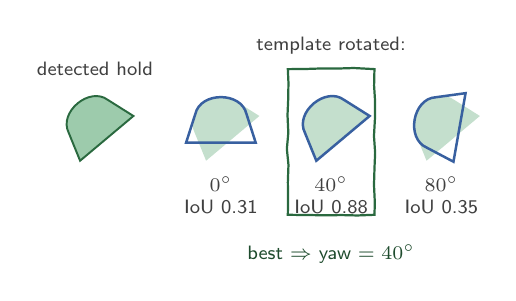
\begin{tikzpicture}
\pgfmathsetseed{9}
\node[note] at (0,1.05) {detected hold};
\pic[rotate=40, fill=cShared!50, draw=cShared!70!black, line width=.7pt, scale=1.3] at (0,0.35) {holdshape};
\foreach \a/\x/\v in {0/1.6/0.31, 40/3.0/0.88, 80/4.4/0.35} {
  \pic[rotate=40, fill=cShared!30, draw=none, scale=1.3] at (\x,0.35) {holdshape};
  \pic[rotate=\a, draw=cSyn!80!black, line width=.9pt, scale=1.3] at (\x,0.35) {holdshape};
  \node[note] at (\x,-0.55) {$\a^\circ$\\IoU \v};
}
\node[note] at (3.0,1.35) {template rotated:};
\node[note, text=cShared!50!black] at (3.0,-1.3) {best $\Rightarrow$ yaw $= 40^\circ$};
\draw[cShared!70!black, line width=.8pt, sketch] (2.45,-0.8) rectangle (3.55,1.05);
\end{tikzpicture}}\\[2pt]
{\footnotesize (c) \textbf{Yaw.} The hold's silhouette is compared with one template hold rotated in $3^\circ$ steps;
the best overlap gives the yaw.}
\end{minipage}
\caption{Three key steps of the detector.}
\label{fig:concepts}
\end{figure}

\textbf{Calibration.} Synthetic: the red square's four corners give a homography pixel $\rightarrow$ meters
(\path{synthetic_wall/calibration.py}); its size comes from \code{scene.json}. The contour corners lie on the
centres of the edge pixels, which makes the square 1--2~px too small; \code{subpixel\_quad()} enlarges them to the
square's soft (anti-aliased) area. This matters for a small marker: on wall~4 (0.1~m marker, 65~px) it was a 2.7\% scale
error, up to 4~cm at the top of the wall. Real: small dark dots on plain
board are found, given integer grid cells and grown into a lattice with a homography fit, 20~cm per cell
(\path{real_wall/grid_calibration.py}). Each image is then resized to a fixed px/m, so a superpixel size in pixels
means the same on every wall. The result is saved as \path{outputs/<wall>/calibration.npz} (the homography
\code{H\_pixel\_to\_m}, \code{px\_per\_m}, the origin and corners; real walls also the grid spacing, angle, wall
extent and residuals). It is the first step of every run: \code{calibrate\_grid.py} for real walls,
\code{calibration.calibrate\_wall()} for synthetic ones (called by \code{run\_wall.run} and the sweep, once per wall
before the parallel runs). Detection and the sweep only read it, with plain \code{np.load}.

\textbf{Hold candidates} (\code{hold\_candidates()} in \path{shared/candidates.py}), the core of the detector. For
each superpixel the code takes its mean Lab color and its Lab distance (the \emph{contrast}) to the \emph{median} color
of the superpixels in a 36~px window, so the holds do not shift the wall color. Superpixels with contrast $>T$ are
kept, cleaned by opening/closing and grouped into blobs. A blob is a hold if its area, aspect ratio and solidity fit a
hold and its saturation is at least $S$; the floor $S$ removes shadows and gray volume faces.

\textbf{Type, position, yaw, depth.} Type is the nearest simulator hue (synthetic) or nearest labelled color in Lab
(real). Position is the blob centroid through the homography. Synthetic yaw: the hold's silhouette is compared with a
template hold rotated in $3^\circ$ steps (intersection over union, \code{orientation.py}); real yaw: the direction of
the longest straight edge. Roll and pitch are written as 0. Depth: the detector runs on both stereo eyes, holds are
matched by color along the epipolar line and triangulated; since the error grows with the squared distance, $z$ is
used only if its expected error is $\le5$~cm, otherwise $z=0$ (\code{final\_output.py}).

\textbf{The three algorithms} get a $3\times3$ blur and 10 iterations, single-threaded (multithreaded LSC is not
deterministic). SLIC (SLICO) is k-means on (Lab, position) in a local window \cite{slic}; LSC is weighted k-means that
approximates normalized cuts \cite{lsc}; SEEDS moves block borders of a coarse grid to improve a color-histogram energy
\cite{seeds}. The size $s$ is the region size for SLIC/LSC and gives area$/s^2$ superpixels for SEEDS. Fig.~\ref{fig:sp} shows the three on the same patch.

\begin{figure}[!htb]
\centering
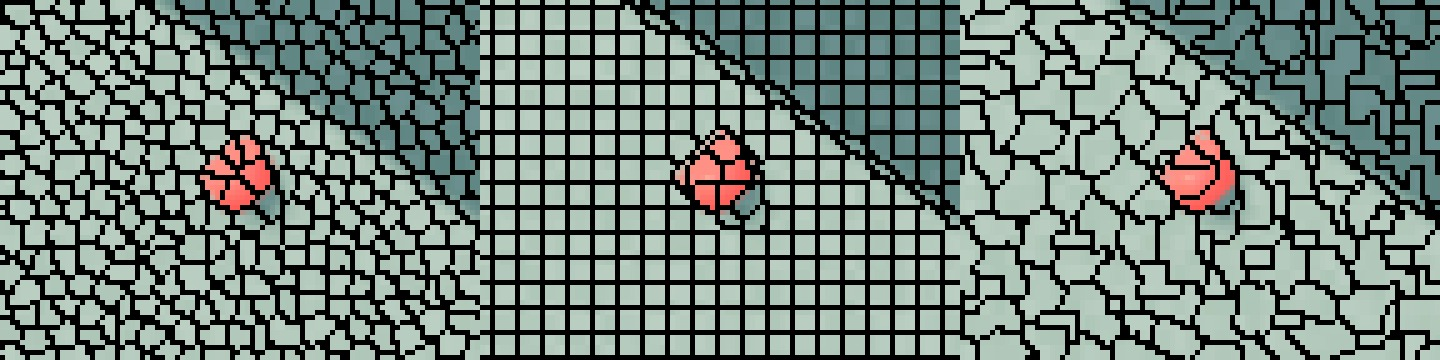
\includegraphics[width=0.85\linewidth]{synthetic_wall_superpixels.jpg}
\caption{The same patch (a hold next to a pyramid) under SLIC, LSC and SEEDS, size 5. SLIC cells are compact and
follow the hold; LSC is almost a regular grid; SEEDS gives irregular blocks.}
\label{fig:sp}
\end{figure}

\textbf{Output} (\path{outputs/<wall>/<algo>/output.json}), one entry per hold, meters and radians; origin at the
bottom-left of the red square (synthetic) or the bottom-left bolt hole (real), $x$ right, $y$ up, $z$ out of the wall:
\begin{cmd}
{"type": "#F2554E", "position": {"x": -0.885, "y": 0.813, "z": 0.0},
 "orientation": {"roll": 0.0, "pitch": 0.0, "yaw": 0.681}}
\end{cmd}
Next to it: \code{score.json} (comparison with the ground truth), \code{detections.png}, \code{superpixels.jpg},
\code{mask.png} and \code{run.log}.

%==========================================================================
\section{Choosing the parameters: the sweep}
\label{sec:params}
Three values are tuned per algorithm: the superpixel size $s$, the contrast threshold $T$ and the saturation floor
$S$. The sweep (\path{pipelines/*/sweep.py}) tries every combination and counts the result against the ground truth:

\begin{center}\small
\begin{tabular}{lL{6.4cm}L{6.6cm}}
\toprule
 & Synthetic & Real\\
\midrule
grid & 3 algorithms $\times$ sizes 3--14 (7) $\times$ $T=10\ldots100$ (19) $\times$ $S\in\{0,118\}$ & the same, with
 $S\in\{0,60,118\}$\\
settings & 798, each on 4 walls (walls 1--3 chose the current baseline) & 1197, tuned on \path{real_wall2}, tested on \path{real_wall1}\\
\bottomrule
\end{tabular}
\end{center}

\begin{figure}[!htb]
\centering
\resizebox{\linewidth}{!}{%
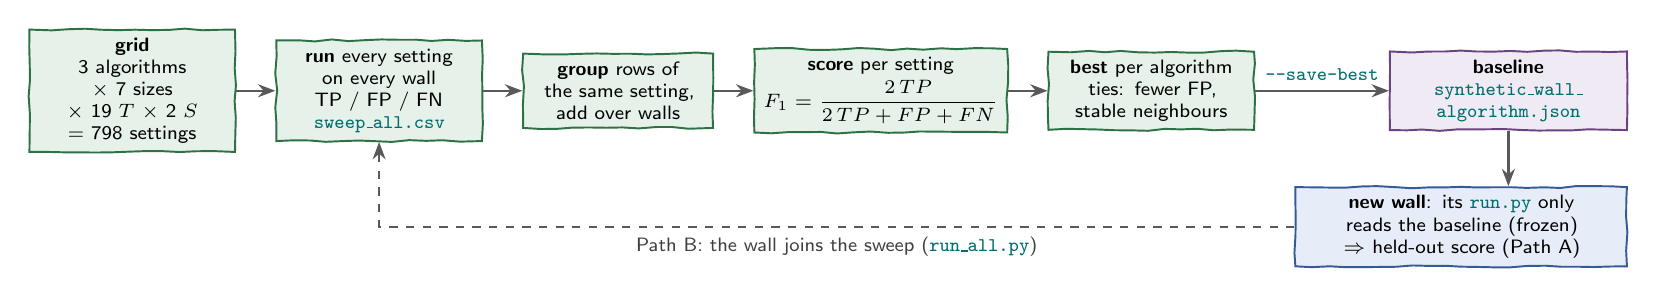
\begin{tikzpicture}
\pgfmathsetmacro{\w}{24}
\pgfmathsetseed{11}
\node[box=cShared, text width=24mm] (g1) {\textbf{grid}\\3 algorithms $\times$ 7 sizes\\$\times$ 19 $T$ $\times$ 2 $S$\\= 798 settings};
\node[box=cShared, text width=24mm, right=5mm of g1] (g2) {\textbf{run} every setting\\on every wall\\TP / FP / FN\\\code{sweep\_all.csv}};
\node[box=cShared, text width=22mm, right=5mm of g2] (g3) {\textbf{group} rows of\\the same setting,\\add over walls};
\node[box=cShared, text width=30mm, right=5mm of g3] (g4) {\textbf{score} per setting\\[1pt]$F_1=\dfrac{2\,TP}{2\,TP+FP+FN}$};
\node[box=cShared, text width=24mm, right=5mm of g4] (g5) {\textbf{best} per algorithm\\ties: fewer FP,\\stable neighbours};
\node[box=cOut, text width=28mm, right=17mm of g5] (g6) {\textbf{baseline}\\\code{synthetic\_wall\_}\\\code{algorithm.json}};
\node[box=cSyn, text width=40mm, below=7mm of g6.south east, anchor=north east] (g7) {\textbf{new wall}: its \code{run.py} only\\reads the baseline (frozen)\\$\Rightarrow$ held-out score (Path A)};
\draw[arr] (g1) -- (g2); \draw[arr] (g2) -- (g3); \draw[arr] (g3) -- (g4); \draw[arr] (g4) -- (g5);
\draw[arr] (g5) -- node[above, note] {\code{--save-best}} (g6);
\draw[arr] (g6) -- (g6 |- g7.north);
\draw[arr, dashed] (g7.west) -| node[pos=0.25, below, note] {Path B: the wall joins the sweep (\code{run\_all.py})} (g2.south);
\end{tikzpicture}}
\caption{From the sweep to a baseline. A setting is one combination of algorithm, size $s$, threshold $T$ and
saturation floor $S$; it is scored on all walls together.}
\label{fig:sweep}
\end{figure}

\label{sec:select}
\textbf{From sweep rows to a baseline} (Fig.~\ref{fig:sweep}) (synthetic; the real sweep is the same on the labelled photo only):
\begin{enumerate}\setlength\itemsep{0pt}
\item \textbf{Count.} A detection within 10~cm of an unmatched true hold is a true positive (TP), any other is a false
positive (FP), an unmatched true hold is a miss (FN) (\code{match()} in \path{shared/matching.py}).
\item \textbf{Group and add.} Rows with the same (algorithm, $s$, $T$, $S$) differ only in the wall; their TP, FP, FN
are added (\code{pooled()}). Example: SLIC, 8, 40, 118 gives 9/0/1, 5/1/2, 6/0/4 on walls 1--3, total 20/1/7.
\item \textbf{Score.} Each group gets $F_1 = 2\,\mathrm{TP}/(2\,\mathrm{TP}+\mathrm{FP}+\mathrm{FN})$; above $40/48=0.83$.
\item \textbf{Pick.} Per algorithm the group with the best $F_1$ wins; ties go to fewer false positives, then to the
higher $F_1$ of the neighbouring thresholds (\code{rank()}, \code{choose()}). The best of the three is \code{best\_algorithm}.
\end{enumerate}

\textbf{ROC curve.} The crucial parameter is $T$: each threshold gives one point (false positives, recall), and the
line is the best recall reachable with at most $k$ false positives (Fig.~\ref{fig:roc}). A false-positive \emph{rate}
is not defined here, since there is no fixed set of non-holds.

\textbf{Frozen baselines.} The baseline files change only with \code{--save-best}. A wall's own \code{run.py} only
reads them, so a wall added later is scored with values that never saw it (a held-out score).

\begin{center}\small
\begin{tabular}{lccccc@{\hspace{2em}}lcccc}
\toprule
\multicolumn{6}{l}{\textbf{Synthetic baseline} (chosen on walls 1--3, 27 holds)} & \multicolumn{5}{l}{\textbf{Real baseline} (chosen on \path{real_wall2})}\\
 & $s$ & $T$ & $S$ & found / FP & $F_1$ & & $s$ & $T$ & $S$ & $F_1$\\
\midrule
SLIC (best) & 8 & 40 & 118 & 20 / 1 & 0.83 & SLIC & 4 & 60 & 60 & 0.74\\
LSC         & 3 & 10 & 0   & 19 / 1 & 0.81 & LSC (best) & 5 & 65 & 60 & 0.77\\
SEEDS       & 3 & 30 & 0   & 21 / 6 & 0.78 & SEEDS & 3 & 70 & 60 & 0.73\\
\bottomrule
\end{tabular}
\end{center}
SLIC leads LSC by 0.02, but on 27 holds one hold is about 0.03 of $F_1$, so the ranking is not significant. The
optimum is also unstable: the calibration fix changed the scale by less than 1\% and moved SLIC's best size from 5
to 8 (before: SLIC 5/40/118, LSC 3/15/0, SEEDS 3/30/118, $F_1$ 0.80/0.80/0.77). Superpixel time at size 8 on the
four walls: SEEDS 2.5~s, SLIC 5.1~s, LSC 16.3~s.

%==========================================================================
\section{Results}
\label{sec:results}
\subsection{Synthetic walls}
Walls 1--3 chose the baselines; \path{synthetic_wall4} was added afterwards with Path~A, so it is a held-out test.

\begin{center}\small
\begin{tabular}{lcccc@{\hspace{2.5em}}lcc}
\toprule
\multicolumn{5}{l}{\textbf{SLIC, per wall}} & \multicolumn{3}{l}{\textbf{Every algorithm}}\\
Wall & found, FP & position & type & yaw (mean / med.) & & 4 walls: found, FP & wall~4 $F_1$\\
\midrule
1 & 9 / 10, 0 & 1.0 cm & 9 / 9 & 13$^\circ$ / 3$^\circ$ & SLIC  & 27 / 37, 1 & 0.82\\
2 & 5 / 7, 1  & 1.6 cm & 5 / 5 & 60$^\circ$ / 72$^\circ$ & LSC   & 24 / 37, 1 & 0.67\\
3 & 6 / 10, 0 & 0.7 cm & 6 / 6 & 5$^\circ$ / 3$^\circ$ & SEEDS & 26 / 37, 6 & 0.67\\
4 (held out) & 7 / 10, 0 & 1.1 cm & 7 / 7 & 28$^\circ$ / 3$^\circ$ & & & \\
all four & 27 / 37, 1 & 1.0 cm & 27 / 27 & 24$^\circ$ / 5$^\circ$ & & & \\
\bottomrule
\end{tabular}
\end{center}

\begin{figure}[!htb]
\centering
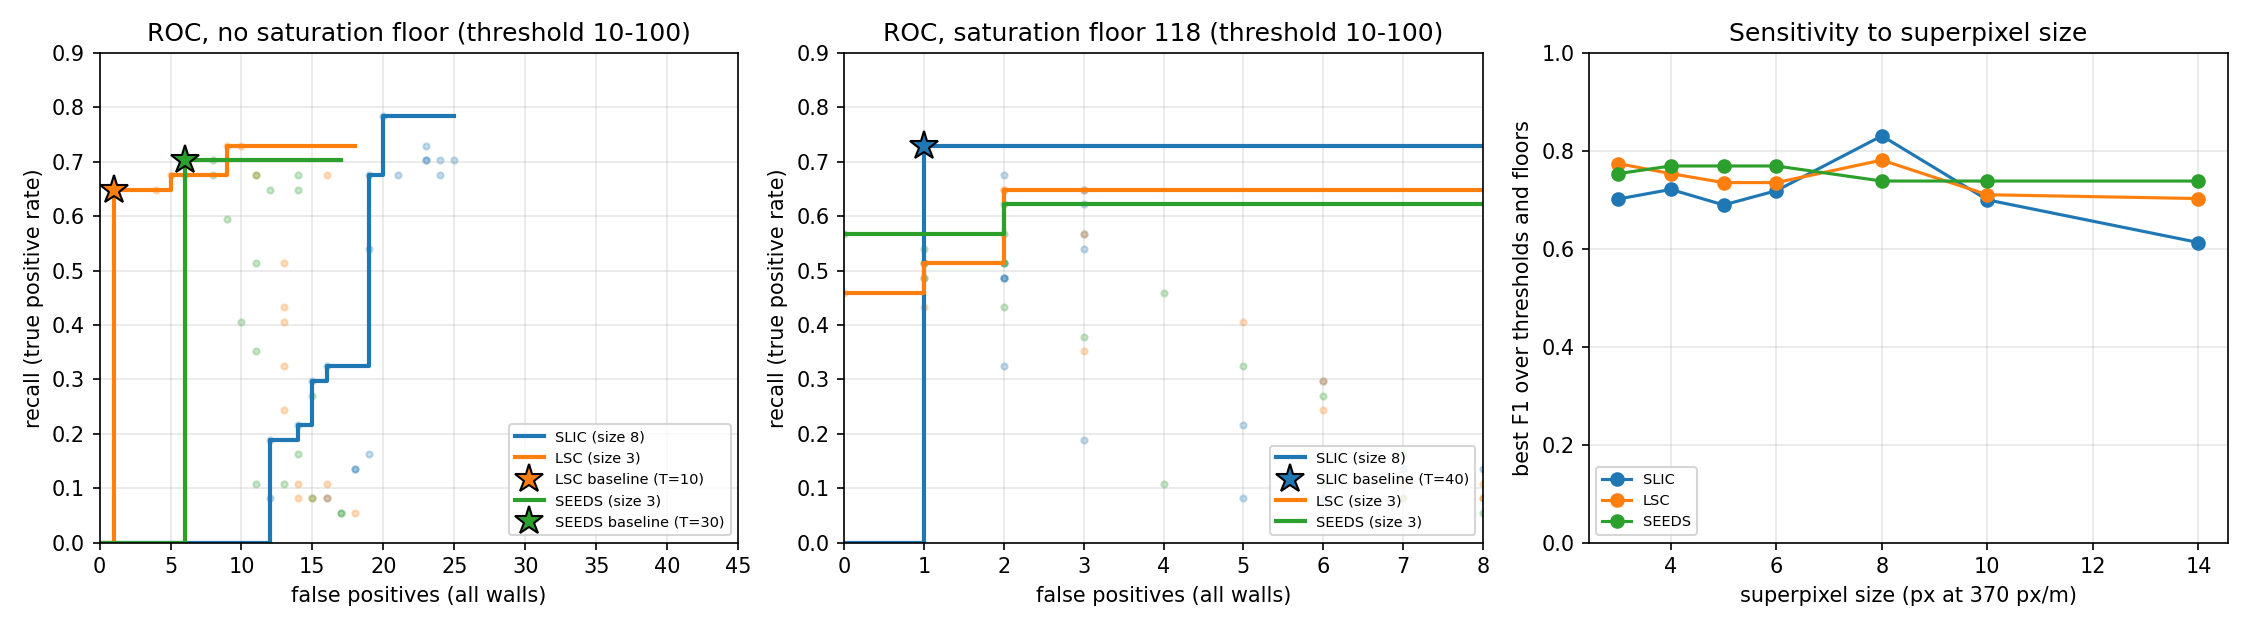
\includegraphics[width=\linewidth]{synthetic_wall_roc_and_sensitivity.png}
\caption{Left, middle: ROC curves from sweeping $T=10\ldots100$, pooled over the four walls, each algorithm at its
baseline size (line: best recall with at most $k$ false positives; dots: single thresholds; stars: baselines).
Right: best $F_1$ against the superpixel size.}
\label{fig:roc}
\end{figure}
\begin{figure}[!htb]
\centering
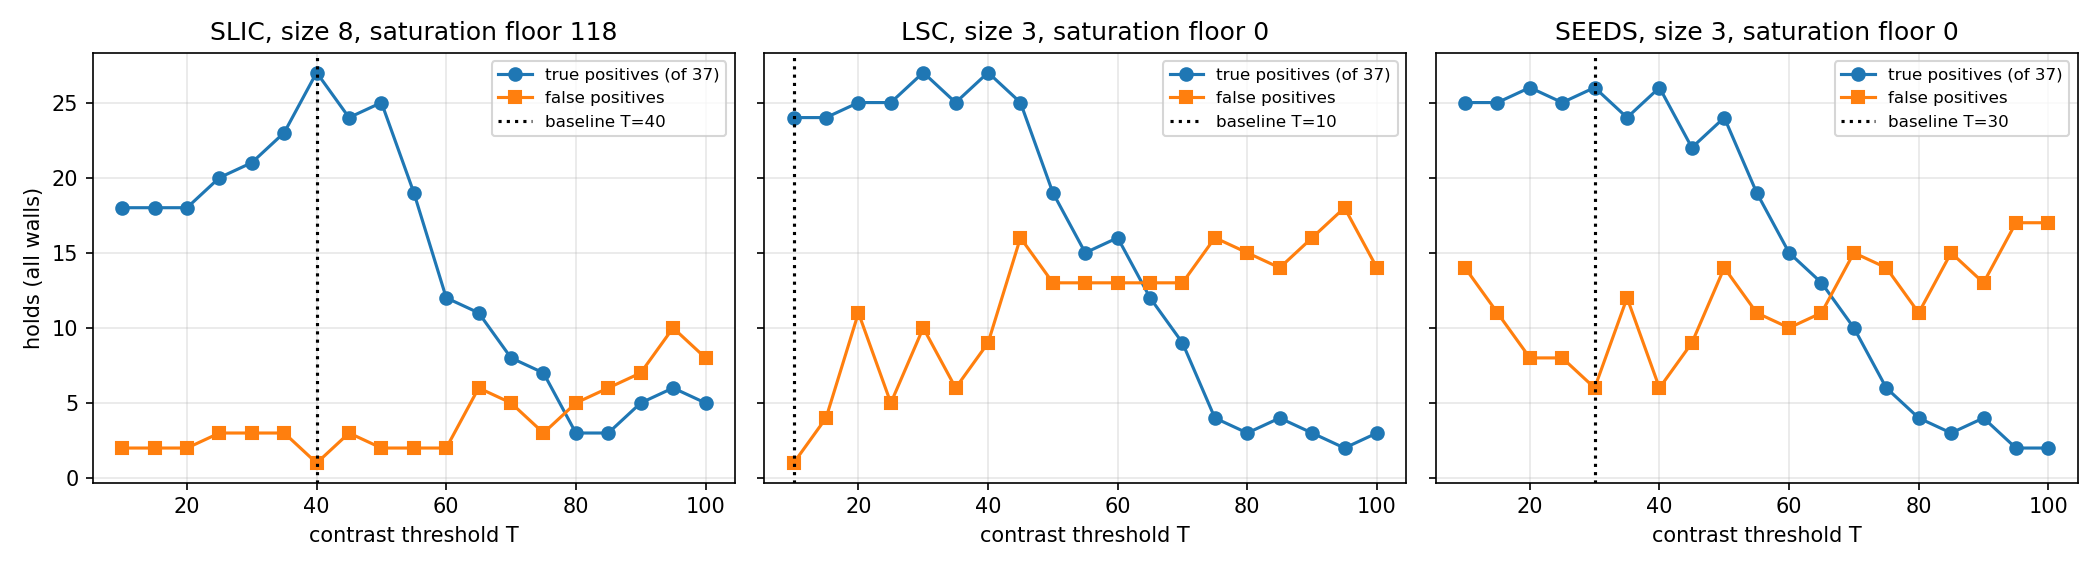
\includegraphics[width=\linewidth]{synthetic_wall_threshold_sensitivity.png}
\caption{Sensitivity to the contrast threshold $T$, each algorithm at its baseline size and saturation floor (four walls).}
\label{fig:thr}
\end{figure}
\begin{figure}[!htb]
\centering
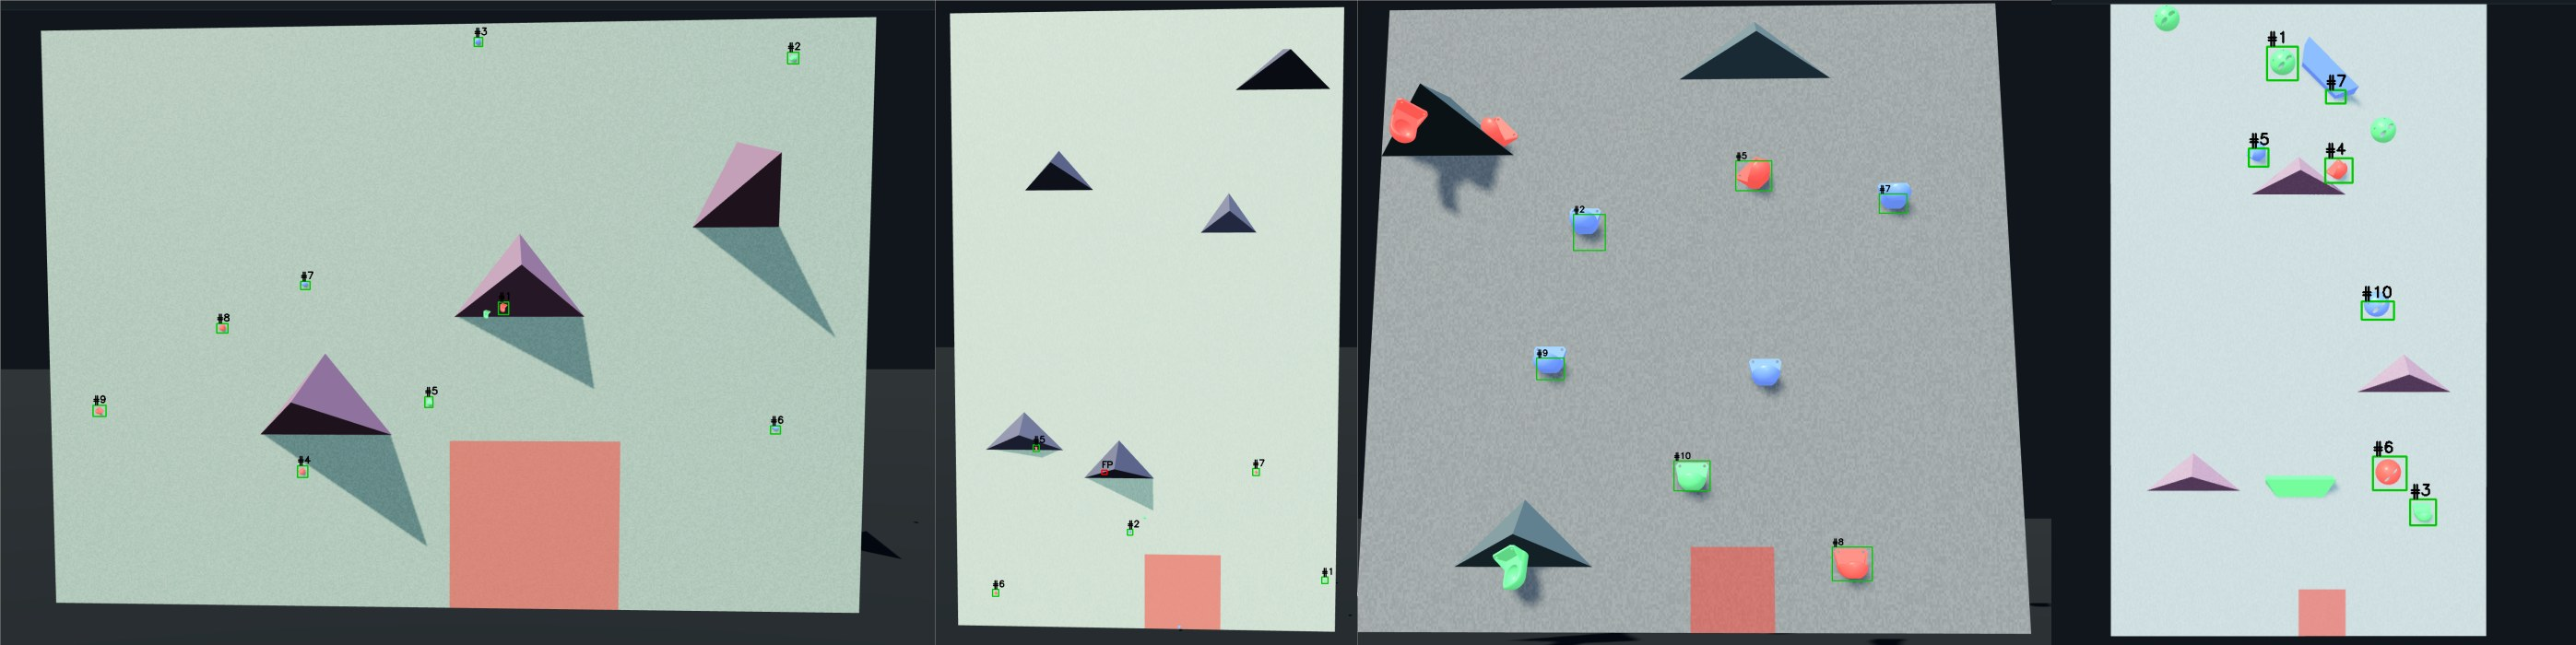
\includegraphics[width=\linewidth]{synthetic_wall_detections.jpg}
\caption{SLIC detections on the four synthetic walls, wall~4 (held out) on the right. Green: matched to a true hold;
red: false positive; uncircled holds are misses.}
\label{fig:det}
\end{figure}

\begin{itemize}\setlength\itemsep{0pt}
\item \textbf{Held-out wall.} With the frozen baselines SLIC finds 7 of 10 holds on wall~4 with no false positive
($F_1$ 0.82, the same as on the tuning walls); LSC and SEEDS find 5 ($F_1$ 0.67).
\item \textbf{The saturation floor matters most.} Without it, reaching 20 of 37 holds costs SLIC 19 false positives
and SEEDS 6; with it SLIC finds 27 with one (Fig.~\ref{fig:roc}). LSC is the exception: it reaches 20 holds with one
false positive without the floor, so its baseline does not use it.
\item \textbf{$T$ is fairly robust:} SLIC keeps 23--27 holds with 1--3 false positives for $T=35\ldots50$ and drops to
12 holds at $T=60$ (Fig.~\ref{fig:thr}). \textbf{The size matters little} between 3 and 10~px (best $F_1$ 0.69--0.78 for
all three), except a peak of SLIC at 8~px (0.83); at 14~px SLIC falls to 0.61, where a superpixel is as large as a hold.
\item \textbf{Type is always right} (color) for the found holds; the position error is 0.7--1.6~cm on walls 1--3 and
1.1~cm on wall~4. \textbf{Yaw} is good on walls 1 and 3 (median $3^\circ$) and fails on wall~2 (holds only 6--7~px
wide). \textbf{Depth} is about 1--2~cm with the camera at 0.75~m (wall~1); at 1--2~m the expected error exceeds 5~cm
and $z=0$.
\item \textbf{Wall 4 brings new hold shapes.} Walls 1--3 contain only \code{microban\_hold}; wall~4 adds
\code{fingerpocket\_hold} (a ball with holes) and \code{sidepull\_hold} (a long bar). The fixed shape filters
(aspect $\le2.5$, solidity $\ge0.85$) were set for microban holds, so the long sidepulls are split or rejected and
fingerpockets with dark holes can fail the solidity test: SLIC's misses are one sidepull and two fingerpockets, and
its only large position error (4.5~cm) is the other sidepull, of which only one end was found. The yaw template is a
microban hold: the microbans get $0$--$3^\circ$ (one $45^\circ$), the other shapes are not meaningful ($63$--$87^\circ$
on two of four).
\end{itemize}

\subsection{Real walls}
\path{real_wall2} (left third of the wall, 100 holds labelled by hand) is the tuning photo; \path{real_wall1} (whole
wall, other camera position) is the test photo, scored inside the region \path{real_wall2} shows. The grid calibration
fits 420 and 238 holes with a median residual of 1~px.

\begin{center}\small
\begin{tabular}{lccccc}
\toprule
 & \multicolumn{2}{c}{\path{real_wall2} (tuning)} & \multicolumn{2}{c}{\path{real_wall1} (test)} & \\
Algorithm & found / FP & $F_1$ & found / FP & $F_1$ & position\\
\midrule
SLIC  & 66 / 13 & 0.74 & 57 / 15 & 0.66 & 3.4--3.9 cm\\
LSC   & \textbf{70 / 13} & \textbf{0.77} & \textbf{60 / 14} & \textbf{0.69} & 3.8--3.9 cm\\
SEEDS & 65 / 14 & 0.73 & 53 / 13 & 0.64 & 3.7--4.3 cm\\
\bottomrule
\end{tabular}
\end{center}

\begin{figure}[!htb]
\centering
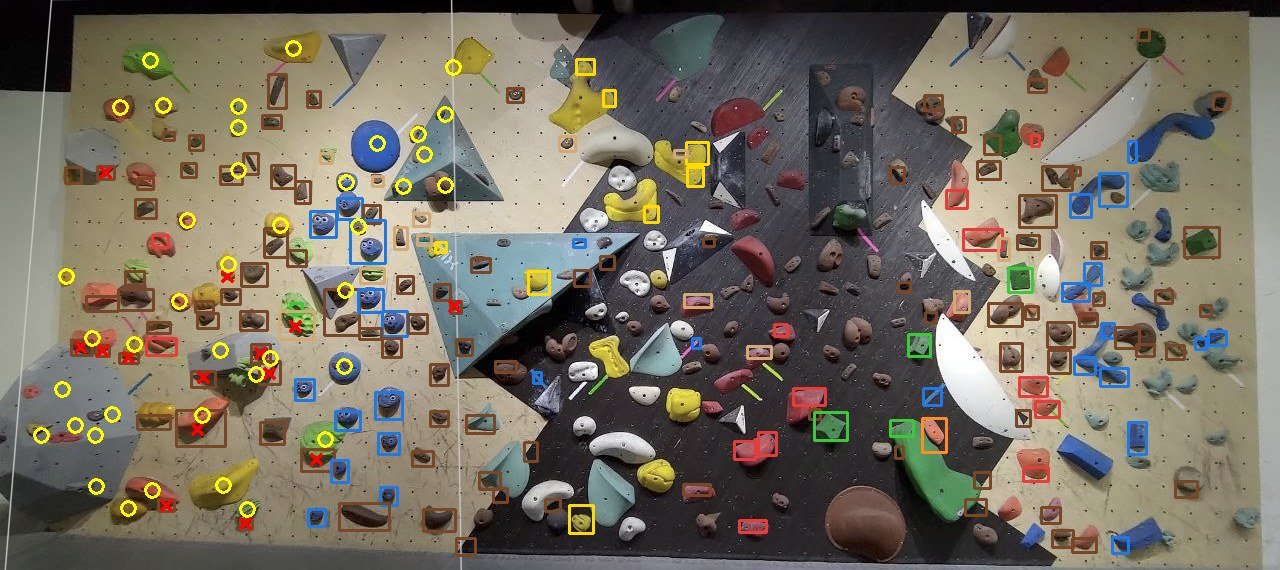
\includegraphics[width=0.48\linewidth]{real_wall_detections.jpg}\hfill
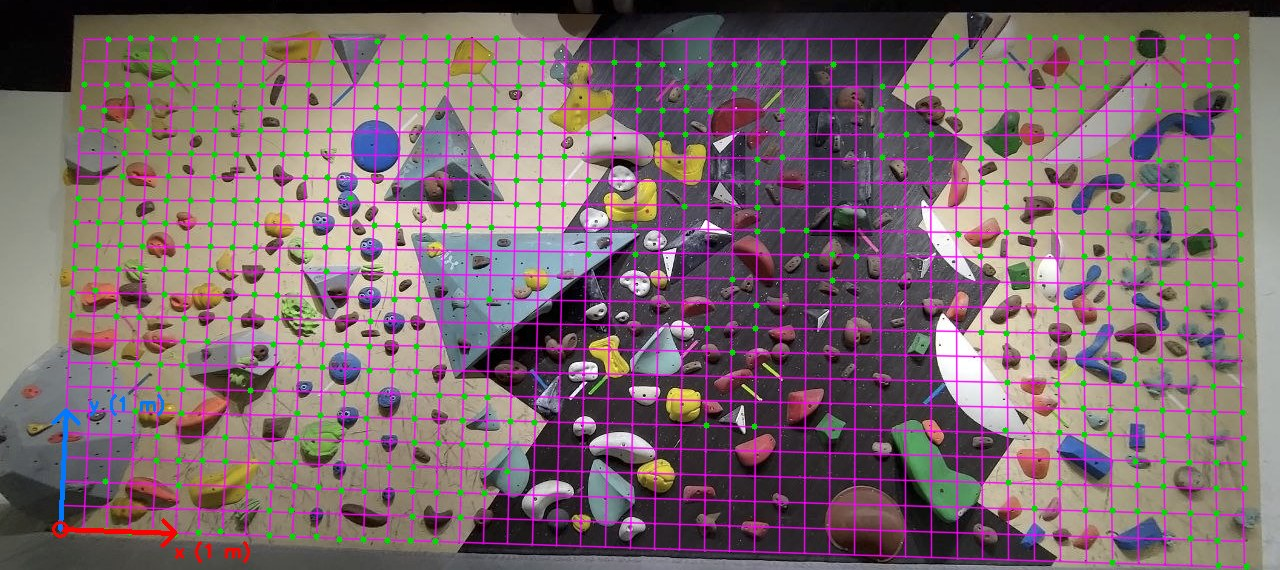
\includegraphics[width=0.48\linewidth]{real_wall_calibration.jpg}\\[3pt]
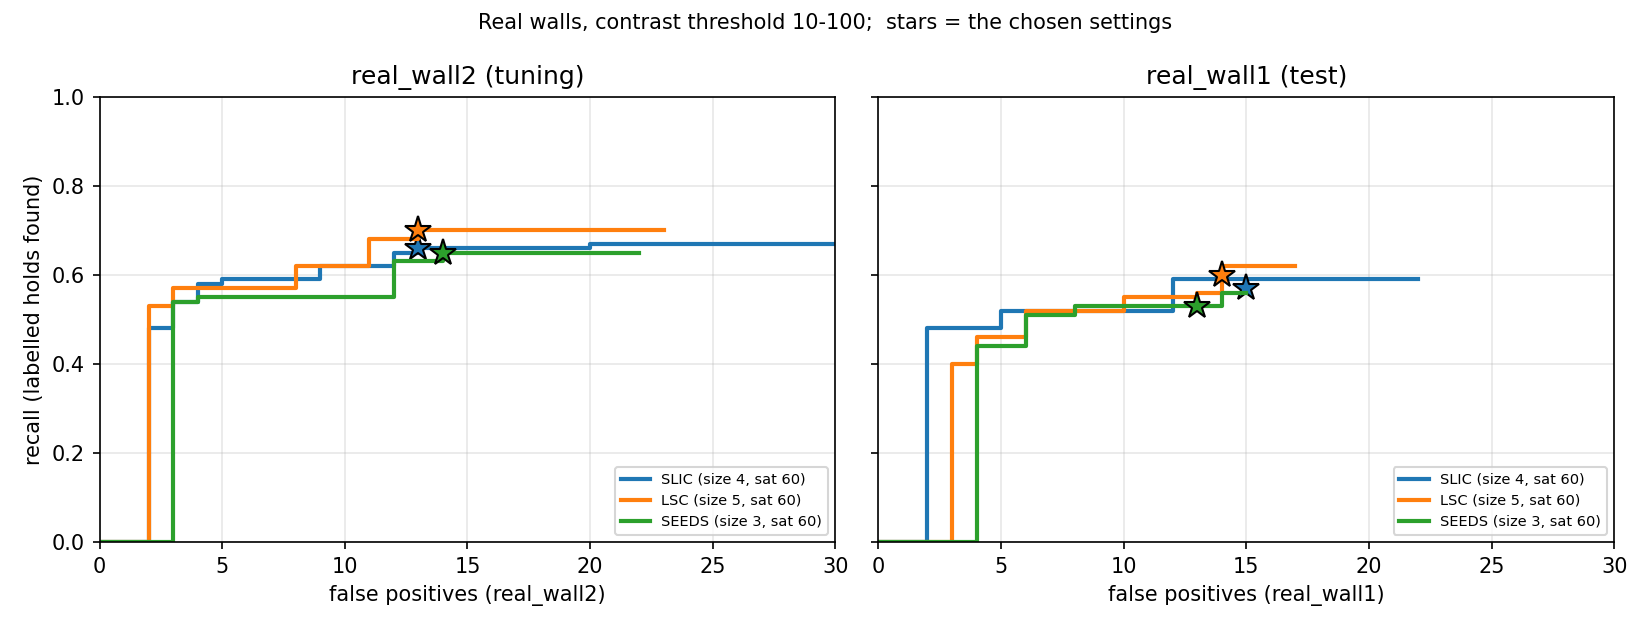
\includegraphics[width=0.75\linewidth]{real_wall_roc.png}
\caption{Top left: \texttt{real\_wall1} with LSC (box color = type, red cross = false positive, yellow circle = missed
labelled hold). Top right: its grid calibration (magenta 20~cm grid, green bolt holes used). Bottom: ROC on the real
photos ($T=10\ldots100$); stars: the chosen settings.}
\label{fig:real}
\end{figure}
LSC is best on both photos, SLIC is close, SEEDS last (Fig.~\ref{fig:real}); all three choose $S=60$. The type agrees
with the labels for 76--77\% of the holds LSC finds, mostly mixing brown, tan and yellow. The optimum is flat: a
0.1\% change of the working scale moved the best thresholds by 5--20 and $F_1$ by up to 0.06, so differences of a few
hundredths are not significant. Yaw has no ground truth on the real walls.

%==========================================================================
\section{Limits and troubleshooting}
\label{sec:trouble}
\begin{itemize}\setlength\itemsep{0pt}
\item \textbf{Little data and optimistic tuning scores.} 27 synthetic holds chose the baseline and are also scored;
an earlier leave-one-wall-out check (before the calibration fix) lowered SLIC's $F_1$ from 0.80 to about 0.70. The
fair number is wall~4 ($F_1$ 0.82 for SLIC, but from only 10 holds). The real labels come from one photo, and the test photo shows the same holds.
\item \textbf{Holds on volumes} are mostly missed, and a found one gets $z=0$ and roll $=0$; roll and pitch are never
estimated. \textbf{Small holds} (5--6~px before resizing) are the weakest case, also for yaw. The yaw template comes
from one hold. Real walls are treated as one plane with $z=0$.
\item \textbf{Hold type means color here.} In \code{scene.json} the \code{type} field is the hold \emph{shape}
(\code{microban\_hold}, \code{fingerpocket\_hold}, \code{sidepull\_hold}); the output gives the color, which was the
only difference between holds on walls 1--3. Classifying shapes, a template per shape and shape-aware filters are
the next step; a wall used to develop them would no longer be a held-out test.
\end{itemize}

\begin{center}\small
\begin{tabular}{L{5.2cm}L{10.4cm}}
\toprule
Symptom & Fix\\
\midrule
\code{red square not found} & export the screenshot again with the whole square visible\\
0 holds on a narrow synthetic wall & check \code{originMarker.width} in \code{scene.json} (0.1~m) or pass \code{--marker}\\
\code{camera.json} not found & add it, or pass \code{--stereo-height} and \code{--stereo-distance}\\
\code{only N grid holes found} & use a larger photo or lower \code{dot\_contrast} in \code{real\_wall\_parameters.json}\\
a sweep does not rerun after an edit & add \code{--force}\\
no module \code{cv2.ximgproc} & install \code{opencv-contrib-python} instead of \code{opencv-python}\\
\bottomrule
\end{tabular}
\end{center}

\begin{thebibliography}{9}\small
\bibitem{slic} R.~Achanta et al., ``SLIC superpixels compared to state-of-the-art superpixel methods,'' IEEE TPAMI, 2012.
\bibitem{lsc} Z.~Li and J.~Chen, ``Superpixel segmentation using linear spectral clustering,'' CVPR, 2015.
\bibitem{seeds} M.~Van den Bergh et al., ``SEEDS: superpixels extracted via energy-driven sampling,'' ECCV, 2012.
\end{thebibliography}

\end{document}
